%!TEX root = ../thesis_a4.tex

\chapter{Music Corpora and Datasets}
\label{chap:corpus_music_corpora_and_datasets}

\TODO{Can't believe a month back I wrote such a shitty text!! many things to be changed}

\section{Introduction}
\label{sec:corpus_intro}

A research corpus is a collection of data compiled to study a research problem. A well designed research corpus is representative of the domain under study. It is practically infeasible to work with the entire universe of data. Therefore, to ensure scalability of information retrieval technologies to real-world scenarios, it is to important to develop and test computational approaches using representative data corpus. Moreover, an easily accessible data corpus provides a common ground for researchers to evaluate their methods, and thus, accelerates the advancement of the knowledge. 

Not every computational task requires the entire research corpus for development and evaluation of approaches. Typically a subset of the corpus is used in a specific research task. We call this subset a test corpus or test dataset. The models build over a test dataset can later be extended to the entire research corpus. Test dataset is a static collection of data specific to an experiment, as opposed to a research corpus, which can evolve over time. Therefore, different versions of the test dataset used in a specific experiment should be retained for ensuring reproducibility of the research results. Note that a test dataset should not be confused with the training and testing split of a dataset, which are terms used in the context of a cross validation experimental setup.

In \gls{mir} a considerable number of the computational approaches follow a data-driven methodology, and hence, a well curated research corpus becomes a key factor in determining the success of these approaches. Due to the importance of a good data corpus in research, building a corpus in itself is a fundamental research task~\citep{macmullen2003requirements}. \Gls{mir} can be still regarded as a relatively new research area within information retrieval, which has primarily gained popularity in last two decades. Even today a significant number of the studies in \gls{mir} use an ad-hoc procedures to build a collection of data to be used for the experiments. Quite often the audio recordings used in the experiments are taken from a researcher's personal music collection. Availability of a good representative research corpus has been a challenge in \gls{mir}~\citep{serra:14:corpus}. This to an extend can be attributed to the large variety of research problems studied within \gls{mir}, lack of standardized methodologies for data collection and annotation, and most of all, due to the constrains posed by the copyrighted content.

In recent years there have been efforts to compile large collections of music related data to build a research corpus that can be used to study a number of computational tasks in \gls{mir}. One such example is the \gls{msd}~\citep{Bertin-Mahieux2011}, which is used in a number of studies for a variety of tasks~\citep{serra2012measuring,sturm2012survey}. However, owing to copyright issues, the audio for the recordings in \gls{msd} is not available. Building a good representative research corpus, which in \gls{mir} would typically mean compiling a large collection of music recordings and it's related metadata is a substantial effort. A successful and sustainable strategy could be to make it a community effort. An endeavor in this direction is AcousticBrainz~\citep{porter2015acousticbrainz}\footnote{\url{https://acousticbrainz.org/}}, which aims to crowd source acoustic information for all music in the world and make it available under public domain. Data in Acousticbrainz is indexed by unique MusicBrainz identifiers. MusicBrainz\footnote{\url{https://musicbrainz.org/}} is an open music encyclopedia that collects music metadata and makes it publicly available. Such open repositories can also serve as corpus for a variety of research problems in \gls{mir}. There have also been some efforts to compile music corpus such as COFLA corpus\footnote{\url{http://www.cofla-project.com/?page_id=170}} in order to perform computational studies of specific music traditions~\citep{kroher2016corpus}.

While there is an increasing effort towards building and using a representative research corpus in \gls{mir}, there are not many studies that address formally the task of building a good research corpus. There is a lack of studies that discuss the criterion for determining the goodness of a corpus for a particular task and systematic ways to compile and curate research corpus. Some recent efforts towards this direction include the work by~\cite{peeters2012towards} in which the authors present a unified way to describe annotated \Gls{mir} datasets. \cite{Humphrey:JAMS:ISMIR:14} define a specifications to store annotations in a more unified way to promote reproducibility and easy access of the corpora. As a part of the CompMusic project \cite{serra:14:corpus} presents a set of design criterion for building research corpora that is representative of a given domain of study. These criterion are based around considerations such as purpose, coverage, completeness, quality and reusability.

In this chapter we describe the CompMusic research corpora built for studying a number of computational tasks in \gls{mir} of \gls{iam}. Before describing the corpora we briefly discuss the methodology and the design criterion used to compile and curate the corpora. Note that the sources used for compiling the corpora are not comprehensive. Our primary aim is to present the approach we used to build the corpora than to justify a specific data source. In addition to the description of the corpora, we also briefly detail the individual test datasets (\secref{sec:corpus_datasets}) built for studying different melodic aspects in \gls{iam}. These test datasets are used for the development and evaluation of different approaches described in the subsequent chapters. 

The compilation of the CompMusic corpora is a collective effort by the CompMusic team. This task mainly involved defining the criterion for selecting music material, procuring audio recordings, entering the associated editorial metadata into the MusicBrainz, organizing and maintaining music collections on the servers, and correcting erroneous metadata with the help of the domain experts. Contributions have been made in all these steps with more focus on the Hindustani music. The description of the CompMusic Corpora and of the design criterion given below is primarily based on the work presented by~\cite{CM_Corpora_Ajay14,serra:14:corpus}.


\section{CompMusic Research Corpora}
\label{sec:corpus_compmusic_research_corpora}

As mentioned in~\secref{sec:context}, the CompMusic project focuses on data-driven computational approaches to describe music recordings and emphasize the use of domain knowledge of a particular music tradition. The project focuses on five different music traditions: Arab-Andalusian (Maghreb), Beijing Opera (China), Turkish makam music (Turkey), Hindustani (North-India) and Carnatic (South-India) music. One of the key ideas in the project is that there are some universal music concepts such as melody and rhythm, which are common across different music traditions. But, many important aspects of a music piece can be better understood and appreciated by focusing on the specificities of the music tradition. Therefore, a significant effort in the CompMusic project has been to compile a representative research corpora that captures the specificities of different music traditions considered in the project. Furthermore, an effort is made to define the criterion that can be used to build and assess a good research corpora. In the subsequent section we describe briefly these design principles.

\subsection{Criterion for Building CompMusic Corpora}
\label{sec:corpus_criterion_for_corpora}

\cite{serra:14:corpus} enumerates a set of design criterion for building a good representative research corpus. These are the principles used in the CompMusic project to build music corpora with which to computationally analyze different music traditions. For this dissertation to be self-contained, we here provide a brief description of these criterion based on the explanation given by~\cite{serra:14:corpus}.

\subsubsection{Purpose}

The purpose for building a data corpus should be clearly specified at the onset. This includes defining the research problems that need to be addressed and the research methodologies that will be used. In the CompMusic project we want to develop methodologies to extract musically meaningful melody and rhythm related features from audio music recordings. The approaches are mostly based on signal processing and machine learning techniques. A research corpus should take these factors into account.

\subsubsection{Coverage}

As mentioned, a good research corpus should be representative of the domain under study. Coverage is a measure of representativeness of a corpus with respect to the concepts to be studied. Given the focus on the quantitative approaches in the CompMusic project, we need sufficient instances of each concept for the data to be statistically significant. For melodic analysis, we need audio recordings and accompanying metadata that represent the diversities present in the melodic aspects of Hindustani and Carnatic music such as different forms, sections, variety of \glspl{raga}, artists from different schools of music, and recordings in different \glspl{shruti}. 

\subsubsection{Completeness}

To successfully use data in a meaningful analyses it should be complemented by appropriate metadata. Completeness indicates the completeness of the associated information or metadata for each audio recording. For the CompMusic corpus it mainly refers to the completeness of the editorial metadata and of the descriptive information accompany each audio recording. 

\subsubsection{Quality}

The quality of the data in a research corpus should be good. In our case it means that the audio should to be well recorded and the accompanying metadata should be accurate. In CompMusic we use commercially produced well recorded audio data and the accompanying information is obtained from reliable sources. However, at times the information even when collected from reliable sources such as editorial metadata on the CD cover is erroneous. In such cases the metadata is validated and corrected with the help of domain experts. 

\subsubsection{Reusability}

Reusability of a corpus is fundamental for reproducibility of the research results. An important aspect that impacts reusability is the ease of access to the corpus. Ideally, a corpus should be easily accessible by the research community and it should be well structured for an easy integration into the work flow. In CompMusic we address the issues regarding reusability and sharing by emphasizing the use of open repositories that are either already suitable or can be easily adapted to our needs. Following this philosophy for organizing editorial metadata we use MusicBrainz. In addition, we make efforts to make the corpus  accessible through a \acrshort{rest}-based Dunya web \gls{api}.

CompMusic corpora for \gls{iam} comprises two corpus; Carnatic music corpus and Hindustani music corpus. We now proceed to describe the specificities of both these corpora. The description will include the type of data that constitute the corpus, the unit of a data sample, selected references for measuring the completeness and coverage of the data and resources for obtaining complementary information about musical concepts. 


\subsection{Carnatic Music corpus}
\label{sec:corpus_carnatic_music_corpus}

\TODO{Why the heck you dont provide a musicbrainz link?, Also talk about bootleg collection!}

\Gls{raga} is the melodic framework and \gls{tala} is the rhythmic framework in both Carnatic and Hindustani music~(\secref{sec:music_background_iam}). They are two key musical concepts in \gls{iam} around which the entire music is composed, performed, organized and taught. As a result of which these concepts have been the main considerations based on which both the corpora are compiled. These corpora primarily comprise audio recordings and its associated editorial metadata. This is the data that is mainly used by the signal processing and machine learning approaches. In addition to that there are lyrics, scores, contextual information on music concepts and community (social) information from online music forums and other sources used mainly for semantic analysis.

While building a representative music corpus there are several considerations specific to the music tradition that are taken into account. For Carnatic music, a concert, also referred as a (Kach\={e}ri), is the natural unit of music performance. It is the unit typically considered for organization and digital distribution of Carnatic music content. Though Carnatic music is improvisatory in nature, it is predominantly based on compositions. Most of the compositions are to be sung, as a result of which, vocal music is dominant in Carnatic music. Even in instrumental music, the lead artist aims to mimic vocal singing~\citep{Viswanathan2004}. Based on these considerations, we consulted expert musicologists and musicians such as T.~M.~Krishna to arrive at a representative audio collection of Carnatic music.

The main institutional reference for building Carnatic music collection bas been the \gls{mma}. The \Gls{mma} was conceived to be the institution that would set the standards for Carnatic music. Since 1929, the \Gls{mma} hosts annual conferences on music, which has eventually lead to the December music festival of Madras, one of the largest cultural events of the world. The \gls{mma} has been driving the scholarly research in Carnatic music since a long time and has thus influenced the evolution of the musical concepts being used. The \gls{mma} has an expert pannel that sets the standards and fix procedures for selecting artists for the music festival. Since a long time the \gls{mma} has been recording Carnatic music performances and its archive is considered as one of the main references for Carnatic music. However, the archive is not openly available online. We therefore procured the audio recordings through other commercial sources while following the musical criterion used by the \gls{mma}. We started by collecting the releases of the artists who have performed in the \gls{mma} in the last five years. Subsequently, we expanded the collection to include their teachers and other musicians popular in their era. 

One of the main record labels that specializes in Carnatic music recordings is Charsur, which has been publishing high quality commercial CDs for over 15 years now. The core of the Carnatic music audio collection is from their catalog of music concerts. The details of the corpus in terms of the unique number of recordings, releases, artists, \glspl{raga}, \glspl{tala} and compositions is shown in Figure~\ref{fig:carnatic_corpus_details}. In total, the corpus currently consists of 235~concerts comprising 2380~audio recordings spanning over 500~hours of audio data.

\begin{figure}
	\begin{center}
		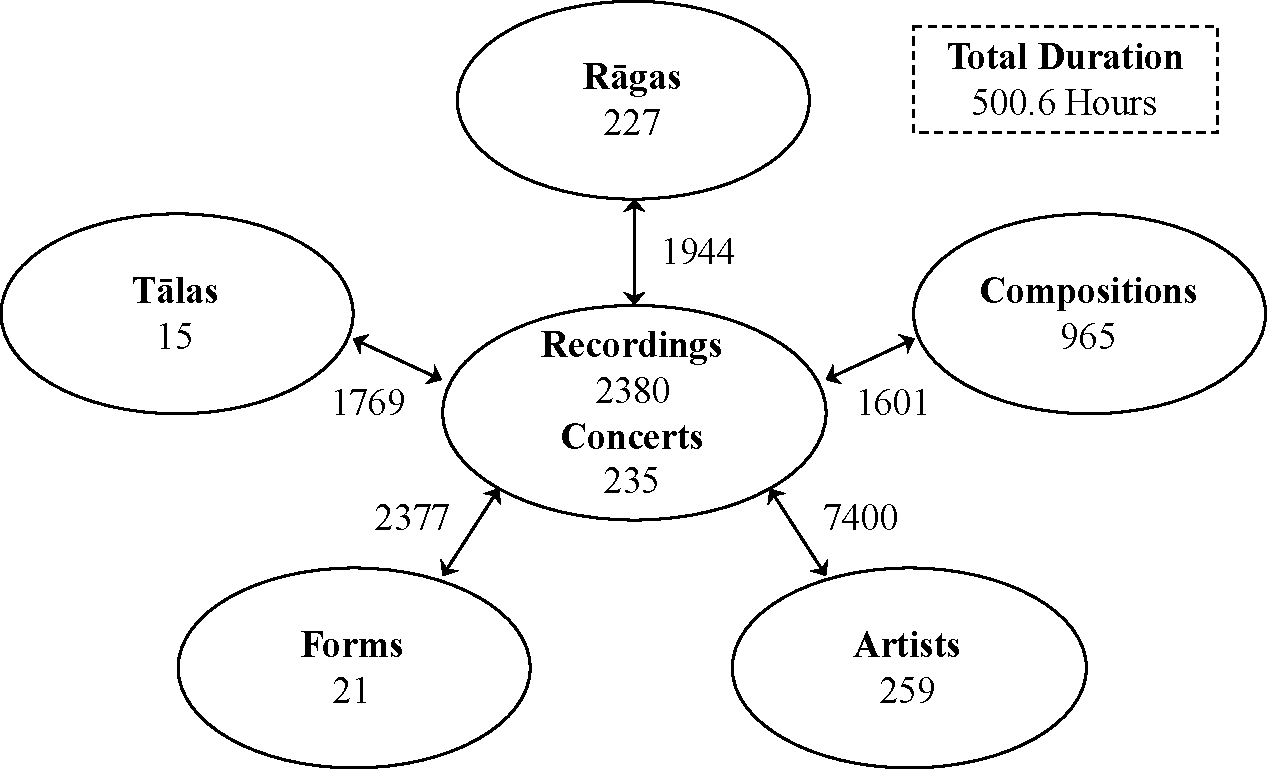
\includegraphics[width=\figSizeNinety]{ch04_datasets/figures/carnatic_corpus_main.pdf}
	\end{center}
	\caption[Details of the Carnatic music corpus]{Details of the Carnatic music corpus in terms of the number of different musical entities and relationships between them.}
	\label{fig:carnatic_corpus_details}
\end{figure}

As mentioned, vocal music constitute a significant part of Carnatic music and it is largely based around compositions. Hence, lyrics play an important role in this music tradition. Scores on the other hand have a limited usability as the music is primarily improvisatory in nature. Nonetheless, for some computational analyses lyrics and scores might be useful, and hence, we make an effort to compile a small collection of them. For most of the currently performed compositions there exists several published compilations of lyrics and scores, for example the ones by the three most recognised composers; Tyagaraja~\citep{TKG_Rao_Tyagaraja}, Syama Sastri~\citep{TKG_Rao_syama} and Dikshitar~\citep{TKG_Rao_Muddusvami}. However, this data is not available in machine readable format and hence is not directly accessible for computational analysis. There are some good open repositories of lyrics such as sahityam.net\footnote{\url{http://sahityam.net/wiki/Main_Page}} that provide lyrics in machine readable format. Sahityam.net is considered as a wikipedia of lyrics of Carnatic music and is our primary source for lyrics. It currently hosts lyrics for about 1820 compositions of Carnatic music. Sources that provide music scores of Carnatic music in a machine readable format are scarce. A compilation of scores done by Dr.~Shivkumar Kalyanaraman\footnote{\url{http://www.shivkumar.org/}} is our main source of scores for Carnatic music.

In addition to the signal processing and machine learning based approaches, semantic analysis of \gls{iam} has been another topic of research in the CompMusic project. The music community and music concepts related information collected from various sources over the Internet comprise the input data to semantic anlaysis and is a part of the Carnatic music corpus. Kutcheries.com\footnote{\url{http://www.kutcheris.com/}} and Wikipedia\footnote{\url{https://en.wikipedia.org/wiki/Category:Carnatic_music}} are two sources utilized for obtaining such an information. Kutcheries.com is a good source of artist biographies and up-to-date information about music venues, concerts and other related events. The category of Carnatic music on Wikipedia is a good source of contextual information including music concepts. There has also been an effort to contribute to Wikipedia by adding information with the help of domain experts. In addition to these two sources, more opinion like data on different musical aspects is obtained from Rasikas.org\footnote{\url{http://www.rasikas.org}}, an active music forum dedicated to Carnatic music community. For the case of Carnatic music the data from rasikas.org can be considered as ideal for studying tasks such as community profiling.


\subsubsection{Coverage of Carnatic Music Corpus}
\label{sec:corpus_coverage_of_carnatic_music_corpus}

Coverage analysis of a corpus aims to measure the representativeness and comprehensiveness of a corpus with respect to the reference sources that represent real-world collections. For the case of the Carnatic music corpus coverage analysis is performed for \glspl{raga}, \glspl{tala}, performing artists and composers. Kutcheris.com is our primary source for measuring artist coverage since it is up-to-date with current artists and their performances. We use last 5 years of their concert listing from 2009-2014. Release catalog from Charsur, our main reference as a record label also provides information about \glspl{raga}, \glspl{tala}, artists and composers. Raaga.com\footnote{\url{http://play.raaga.com/carnatic}}, an Indian music streaming service with a channel dedicated to Carnatic music is another source we considered for this analysis. It should be noted that Raaga.com has several light music forms included in their Carnatic music channel, which we have purposefully not included in our corpus. Hence, the numbers derived from an analysis done on the data from Raaga.com will have an adverse influence because of these additional music forms. The procedure followed for obtaining information from these sources and the post-processing done before the analysis is explained in the article by~\cite{CM_Corpora_Ajay14}.

For each music entity we define a coverage measure, the \textit{overlap} ($O$) as:

\begin{equation}
	O_{e}^{r} = \frac{ | S_{e}^{c} \cap S_{e}^{r} | }{ | S_{e}^{r} |}
	\label{eq:coverage_measure}
\end{equation}

\noindent where $O_{e}^{r}$ is the \textit{overlap} measure of the musical entity $e$ with respect to the reference source $r$, $S_{e}^{c}$ is the set of entities in the corpus and $S_{e}^{r}$ is the set of entities in the reference source. $|S|$ denotes the cardinality of a set $S$. In Table~\ref{tab:coverage_summary_carnatic_corpus} we summarize the coverage of the musical entities along with the overlap measure with respect to the reference sources mentioned above. We see that the coverage of the \glspl{raga} in the corpus is satisfactory and of the \glspl{tala} is good. For composers and artists the numbers are low when compared to Raaga.com, which can be attributed to the presence of light Carnatic music forms in their database. 

\begin{table}
\begin{centering}
\begin{tabular}{ c c c c c }
	\hline
					 & Corpus	& Raaga.com			& Kutcheris 	& Charsur\\
	\hline
	\Glspl{raga}	& 	246		& 	489 (42\%)		& 	N/A			& 301 (68\%)\\
	\Glspl{tala}	& 	18		& 	16 (100\%)		& 	N/A			& 21 (85\%)\\
	Composers		& 	131		& 	598 (17\%)		& 	N/A			& 256 (42\%)\\
	Artists			& 	233		& 	501				& 	2978		& 264 (48\%)\\						
	\hline
	
\end{tabular}
\par \end{centering}	
\caption[Coverage of the Carnatic music corpus]{Summary of the coverage of the Carnatic music corpus. The numbers in the paranthesis indicate the computed \textit{overlap} measure. N/A denotes data not available.} 
\label{tab:coverage_summary_carnatic_corpus}
\end{table}

Not all the performing artists in the corpus (\tabref{tab:coverage_summary_carnatic_corpus}) are lead artists. Among these 233 artists 74 are lead artists (lead vocal or lead instrumental), 28 are accompanying violinists and 48 are percussionists. Since Carnatic music corpus predominantly comprises vocal music, coverage of lead or vocal artists becomes more important. Also not every lead artist is equally popular, that should also be a consideration in measuring the representativeness of the corpus. The concerts listed by Kutcheris.com span the whole year and all through the day. However, the evening concerts are more
recognized, and we took that to be a measure of the popularity of an artist. For a better coverage analysis, we thus consider three categories of artists: Artists-Set-1 (all the artists), Artists-Set-2 (artists who have performed in the evening concerts, through the year) and Artists-Set-3 (artists who
have performed in evening concerts between November and January). Of the 2978 total artists present in Set-1 on Kutcheris.com concert listings, there are 1814 artists in Set-2 and 1472 artists in Set-3.

\begin{figure}
	\begin{center}
		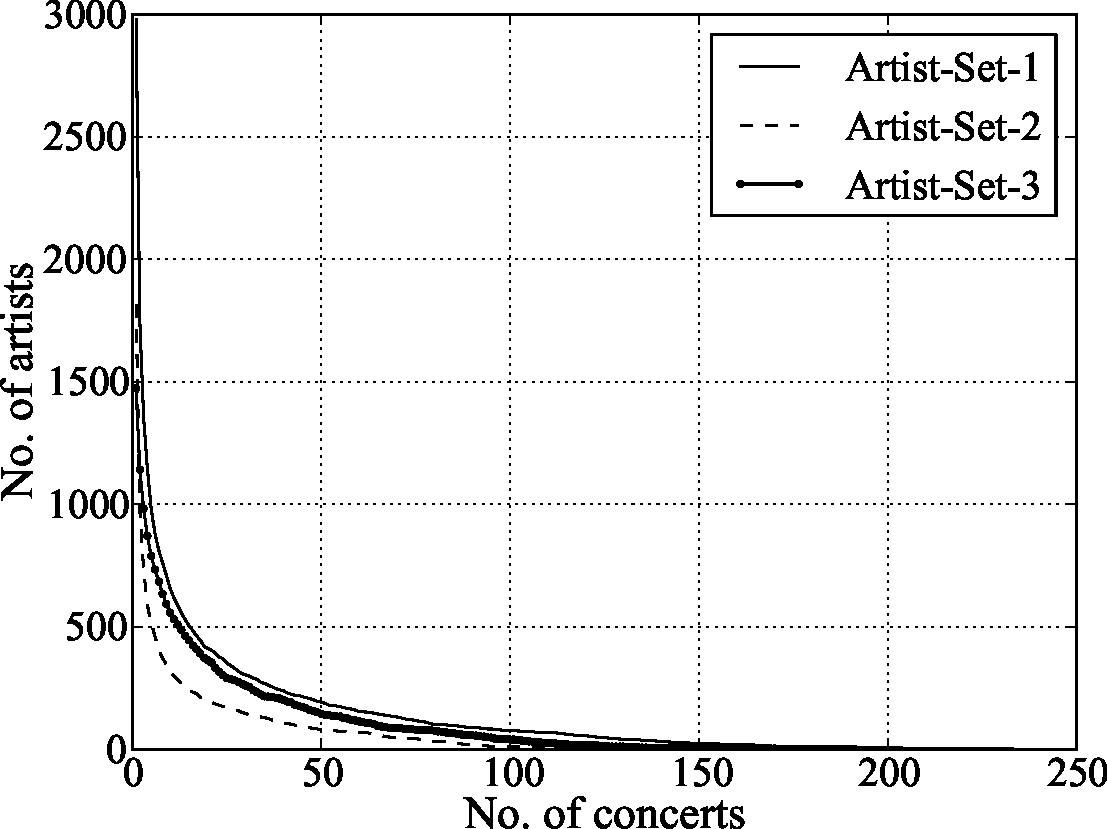
\includegraphics[width=\figSizeEighty]{ch04_datasets/figures/performances-vs-artists.pdf}
	\end{center}
	\caption[Number of artists versus number of concerts]{The number of artists versus number of their concerts. These artists are the ones obtained from Kutcheris.com}
	\label{fig:number_artrist_vs_number_concerts}
\end{figure}

In addition to the timing of the concerts, popularity of an artist can also be measured based on the number of concerts. Though there are a large number of artists listed in Kutcheris.com, we notice that the distribution of the number of concerts they have performed is exponential (\figref{fig:number_artrist_vs_number_concerts}). We see that there are only about 200 artists of 2978 artists who have performed in over 50 concerts. To consider this aspect while measuring coverage, we compute the \textit{overlap} as defined in \eqref{eq:coverage_measure} through different subsets of the artists in Kutcheris.com, sweeping over the number of concerts they have performed. Furthermore, we perform this analysis for different categories of the artists in the corpus as mentioned above.

\begin{figure}
	\begin{center}
		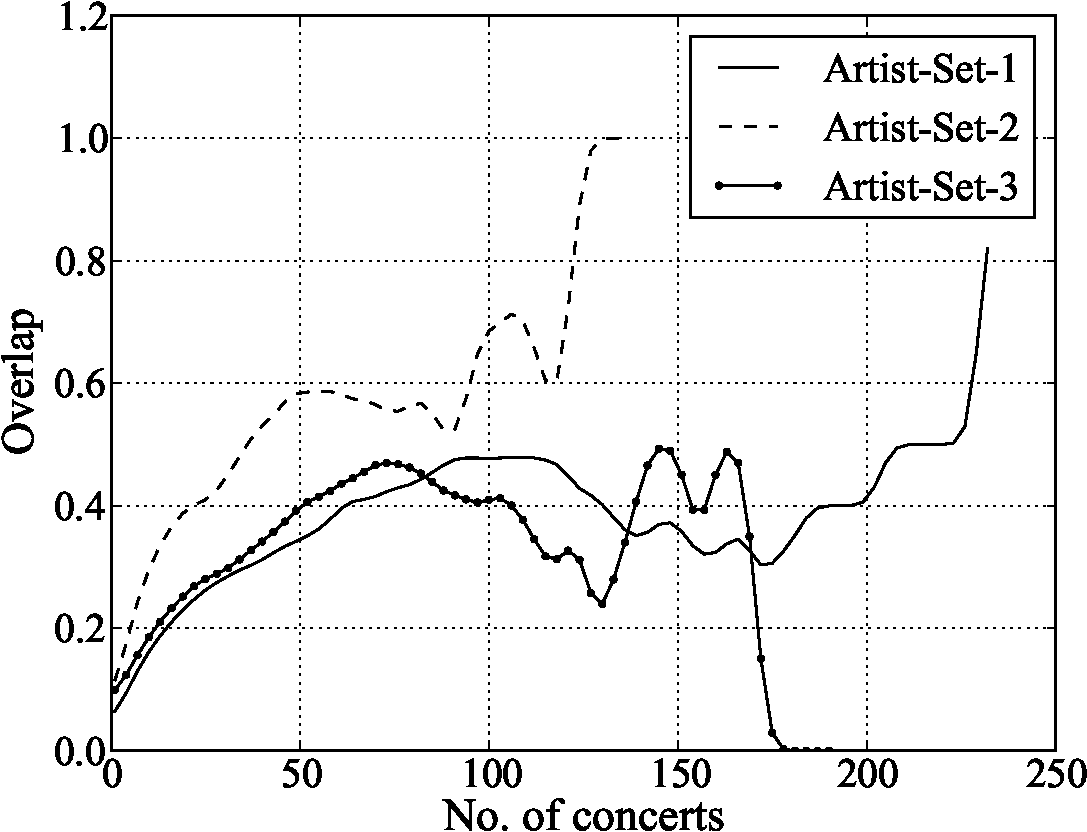
\includegraphics[width=\figSizeEighty]{ch04_datasets/figures/artist-coverage-vs-performances.pdf}
	\end{center}
	\caption[Overlap between the artists in the Carnatic music corpus and Kutcheris.com]{The \textit{overlap} between the artists in the corpus and those listed in Kutcheris.com for different artist sets determined by the number of performed concerts. The analysis is performed for every category of artists in the corpus.}
	\label{fig:artist_coverage_vs_number_of_concerts}
\end{figure}

In \figref{fig:artist_coverage_vs_number_of_concerts} we show the \textit{overlap} between the artists in the corpus and the ones listed in Kutcheris.com for different sets of artists based on the number of performed concerts. We compute the \textit{overlap} curve for all three categories of the artists in the corpus. We notice that the \textit{overlap} increases as we consider more frequently performing artists. We also observe that the \textit{overlap} saturates and becomes constant. This can be attributed to the fact that the most frequently performing artists are the accompanists and they are few in numbers compared to the lead artist, as they accompany multiple lead artists. Since the number of artists with more than 150 concerts is very less, the \textit{overlap}
values becomes unreliable. Overall we notice that the \textit{overlap} is better for artists in the category Artist-Set-2 than Artist-Set-1 and Artists-Set-3. This also indicates that the corpus has a better coverage of the artists from evening concerts round the year.


\subsubsection{Completeness of the Canatic Music Corpus}
\label{sec:corpus_completeness_of_completeness_of_carnatic_music_corpus}

As defined earlier, completeness of the corpus in the context of the CompMusic corpora refers mainly to the completeness of the associated metadata
for each recording. The editorial metadata as will be explained in detail (\secref{sec:corpus_storage_and_access}) is stored and accessed from MusicBrainz. There can be multiple reasons for missing and erroneous editorial metadata in the MusicBrainz. Many times commercially released CDs do not provide all the relevant editorial metadata on the cover-art. In several cases there is no mention of the accompanying artists or of the \gls{raga} and \gls{tala} of the musical piece. Very often composition information is missing on the CD cover. Another reason for incomplete metadata can be that the editorial metadata is not completely entered into the MusicBrainz. This happens quite frequently for the fields such as recording relationships. Several times the metadata entered is erroneous. This is either due to a mistake done by the person uploading the metadata into the MusicBrainz or that the editorial metadata provided on the CD cover itself is wrong. Multiplicity of languages used in Carnatic music further adds to these inconsistencies. There has been some effort to automatically complete the missing metadata based on the relationships on the release and the recordings using semantic web approaches. The missing metadata due to transliteration errors also has been addressed to an extent by making curated list of entities such as \gls{raga} and \gls{tala}, and using robust algorithm for matching and linking metadata. Despite these efforts, there are a significant number of recordings and releases for which the metadata is incomplete.


\begin{table}
	\begin{centering}
		\begin{tabular}{ c c c c}
			\hline
			Metadata	 		&  \#Recordings	& completeness (\%)\\
			\hline
			Lead artist			& 	1650	& 	100	\\						
			Accompanying artist	& 	1221	& 	74	\\
			\Glspl{raga}		& 	959		& 	58	\\
			\Glspl{tala}		& 	917		& 	56	\\
			Work (compositions)		& 	989		& 	60	\\
			
			\hline
			
		\end{tabular}
		\par \end{centering}	
	\caption[Completeness of the Carnatic music corpus]{Completeness of the Carnatic music corpus showing the number of recordings for which the corresponding metadata is available and the percentage (\%) of such recordings. The percentage values are rounded off to the nearest integer.} 
	\label{tab:completeness_carnatic_corpus}
\end{table}


In \tabref{tab:completeness_carnatic_corpus} we show the completeness of the recordings in the Carnatic music corpus. We see that all the recordings are at least labeled with a lead artist, but about a quarter of the recordings (429/1650) do not have any accompanying artist information. \Gls{raga}, \gls{tala} and work (composition) labels are available for more than half the number of recordings. Note that there are some recordings that have the required editorial metadata but deemed incomplete because the names could not be accurately matched to any entity in the curated list. 


\subsection{Hindustani Music Corpus}
\label{sec:corpus_hindustani_music_corpus}

Similar to the case of Carnatic music, \gls{raga} and \gls{tala} are the fundamental music concepts with which to describe melodic and rhythmic aspects of Hindustani music. They thus become the primary considerations while building the Hindustani music corpus as well. In Hindustani music also vocal music is predominant. However, compared to Carnatic music instrumental performances in Hindustani music are much more popular and prevalent. Hindustani music tradition as compared to Carnatic music is much more diverse and heterogeneous. One of the reasons for this can be the geographical spread of this music tradition. Hindustani music thus presents a significant challenge in compilation of a good research corpus. Another major difference between the two music traditions is that in Hindustani music the compositions are very short. The compositions basically act as base for improvisation, which is the main focus in a performance of Hindustani music. For compilation of the Hindustani music corpus we focus on two important vocal music styles; Dhrupad and Khy\={a}l (\secref{sec:music_background_iam}). %A Khy\={a}l performance typically has a lead vocals, a melodic accompaniment (typically given by harmonium or s\={a}ra\o{n}gi), a rhythm accompaniment (typically given by tabla) and a drone sound in the background (typically given by a t\={a}npura). 

There are many institutions that have compiled large audio archives of Hindustani music. The prominent ones among them are the \gls{itc-sra}, Sangeet Natak Academy, and the \gls{air}. Each of these institutions own thousands of hours of expert curated music recordings that represent the real world performance practices of Hindustani music. \gls{itc-sra} is a premier music academy of Hindustani music and has taken up major efforts in the archival of music. Sangeet Natak Academy is India’s national academy for music, drama and dance. \gls{air} is the largest public broadcaster in India and has a large archive of Hindustani music curated over many decades. \gls{air} awards grades to performing musicians and its archives can be considered as a reference for Hindustani music. Like in most of the cases, none of these archives is publicly available. In such a situation, we gathered commercially released audio recordings from several music labels and compiled our own corpus using these institutions as a reference. During this process we also consulted expert musicians and musicologists, such as Dr. Suvarnalata Rao at the \gls{ncpa}, Mumbai, India, to curate the audio collection in the corpus. 

The Hindustani music corpus primarily comprises khy\={a}l and dhrupad vocal music releases, though a significant number of instrumental music releases are also present. There are 233 releases with a total of 1096 recordings spanning over 300 hours of audio. The details of the Hindustani music corpus in terms of the unique number of recordings, releases, artists, \glspl{raga}, \glspl{tala} and compositions is shown in \figref{fig:hindustani_corpus_details}.


\begin{figure}
	\begin{center}
		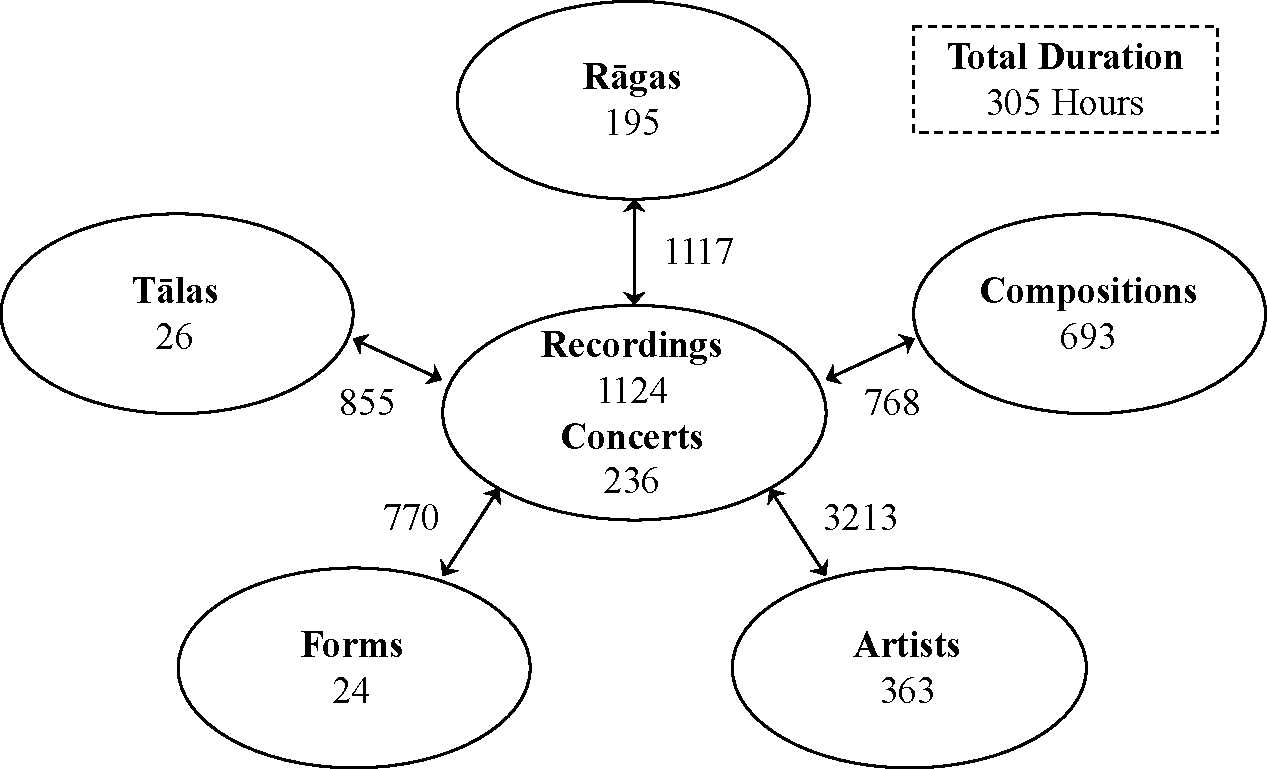
\includegraphics[width=\figSizeNinety]{ch04_datasets/figures/hindustani_corpus_main.pdf}
	\end{center}
	\caption[Details of the Hindustani music corpus]{Details of the Hindustani music corpus in terms of the number of different musical entities and relationships between them}
	\label{fig:hindustani_corpus_details}
\end{figure}


As mentioned before, compositions in Hindustani music are short and they basically act as a base for improvisation. The music performances mainly comprise improvised music material. Due to these factors lyrics and scores are not very relevant for the computational anlaysis of Hindustani music. There exists few repositories such as Bhatkhande~\citep{Bhatkhande_1990} and Ramashray Jha~\citep{R_Jha_2001} who have compiled lyrics and scores of several bandishes (compositions) using a standard notation for Hindustani music. However, they are not available in a machine readable format. In addition to lyrics and scores there are some information repositories such as Swarganga Music Foundation\footnote{\url{https://www.swarganga.org/}} for musical concepts such as \glspl{raga}, \glspl{tala} and bandishes (compositions). The category of Hindustani music on Wikipedia\footnote{\url{https://en.wikipedia.org/wiki/Category:Hindustani_music}} is a good source of contextual information including music concepts of Hindustani music.

\subsubsection{Coverage of Hindustani Music Corpus}
\label{sec:corpus_coverage_of_hindustani_music_corpus}

For the coverage analysis of the Hindustani music corpus we follow exactly the same methodology as was for the Carnatic music corpus. The analysis is done for artists, \glspl{raga}, \glspl{tala} and compositions. Large geographical spread, lack of dedicated record labels and heterogeneous nature of the music make the coverage analysis of Hindustani music more complex compared to Carnatic music. Therefore, it is challenging to do a comprehensive artist coverage analysis like the one presented for Carnatic music. For each of the entities, we choose two main institutional references, \gls{itc-sra} and Swarganga. In  \tabref{tab:coverage_summary_hindustani_corpus} we show the coverage of the Hindustani music corpus. We see that even though the corpus and the chosen references have comparable the number of entities, the \textit{overlap} between them is less. This can be attributed to the differences in the purpose of creating the music collection. We mainly focused on recordings made in last 20-30 years to ensure good recording quality and to reflect current performance practices. On the other hand, both the references focus primarily on archiving Hindustani music and hence consist of several generations of artists, infrequent \glspl{raga} and \glspl{tala}, and a more comprehensive list of compositions. Furthermore, in our Hindustani music corpus we focus on vocal music recordings of only two styles, khy\={a}l and dhrupad. The reference archives additionally include instrumental music and several other styles of Hindustani music.


\begin{table}
	\begin{centering}
		\begin{tabular}{ c c c c}
			\hline
			& Corpus	& ITC-SRA			& Swarganga\\
			\hline
			Artists			& 	360		& 	240 (19\%)	& 	629 (14\%)\\						
			\Glspl{raga}	& 	176		& 	185 (48\%)	& 	534 (13\%)\\
			\Glspl{tala}	& 	32		& 	N/A			& 	59 (37\%)\\
			Works			& 	685		& 	N/A			& 	1957\\

			\hline
			
		\end{tabular}
		\par \end{centering}	
	\caption[Coverage of the Hindustani music corpus]{Coverage of the Hindustani music corpus. The numbers in the parenthesis indicate the computed \textit{overlap} measure. N/A denotes data not available.} 
	\label{tab:coverage_summary_hindustani_corpus}
\end{table}


\subsubsection{Completeness of Hindustani Music Corpus}
\label{sec:corpus_completeness_of_hindustani_music_corpus}

In \tabref{tab:completeness_hindustani_corpus} we show the completeness of the editorial metadata for Hindustani music. We see that the editorial metadata for all the recordings at least includes a lead artist, and for more than half of the collection, the accompanying artists. Roughly 90\% of the corpus is annotated with \gls{raga} label and more than half with \gls{tala} label. Work (bandish) labels are present for nearly half of the collection. \Gls{alap} performances in Hindustani music are completely improvisatory musical pieces and are not based on compositions. Also, they are unmetered in nature, and hence they are not assigned any \gls{tala} label. Ideally, such music pieces should be discounted while assessing the completeness of the work  and the \gls{tala} metadata. Due to unavailability of the \gls{alap} labels on recordings these performances are also included in the assessment and hence work and \gls{tala} completeness is an underestimate.



\begin{table}
\begin{centering}
	\begin{tabular}{ c c c c}
		\hline
		Metadata	 		&  \#Recordings	& completeness (\%)\\
		\hline
		Lead artist			& 	1096	& 	100	\\						
		Accompanying artist	& 	658		& 	60	\\
		\Glspl{raga}		& 	960		& 	88	\\
		\Glspl{tala}		& 	627		& 	57	\\
		Work (Bandish)		& 	576		& 	53	\\
		
		\hline
		
	\end{tabular}
	\par \end{centering}	
\caption[Completeness of the Hindustani music corpus]{Completeness of the Hindustani music corpus showing the number of recordings for which the corresponding metadata is available and the percentage (\%) of such recordings. The percentage values are rounded off to the nearest integer.} 
\label{tab:completeness_hindustani_corpus}
\end{table}


\subsection{Open-access Music Corpus}
\label{sec:corpus_open_access_research_corpus}

\begin{figure}
	\begin{center}
		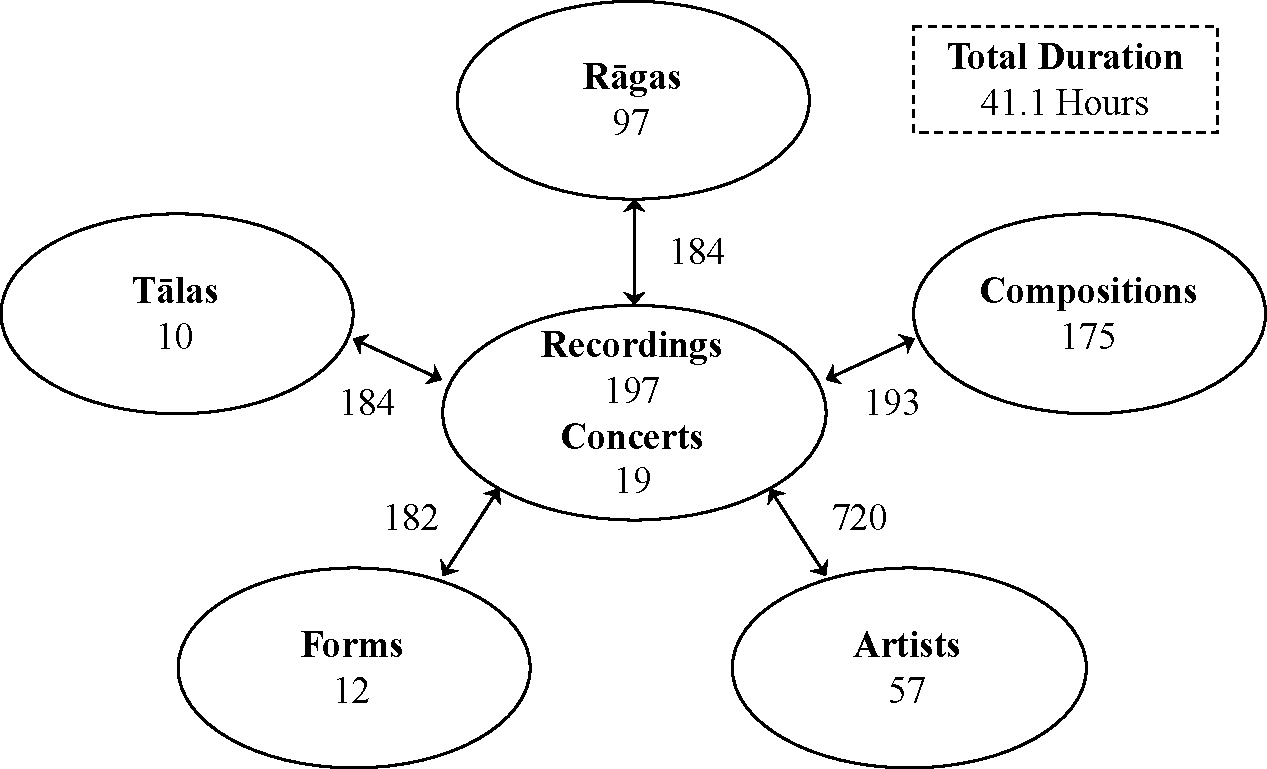
\includegraphics[width=\figSizeNinety]{ch04_datasets/figures/carnatic_corpus_cc.pdf}
	\end{center}
	\caption[Details of the Open-access Carnatic music corpus]{Details of the Open-access Carnatic music corpus in terms of the number of different musical entities and relationships between them}
	\label{fig:carnatic_cc_corpus_details}
\end{figure}

\begin{figure}
	\begin{center}
		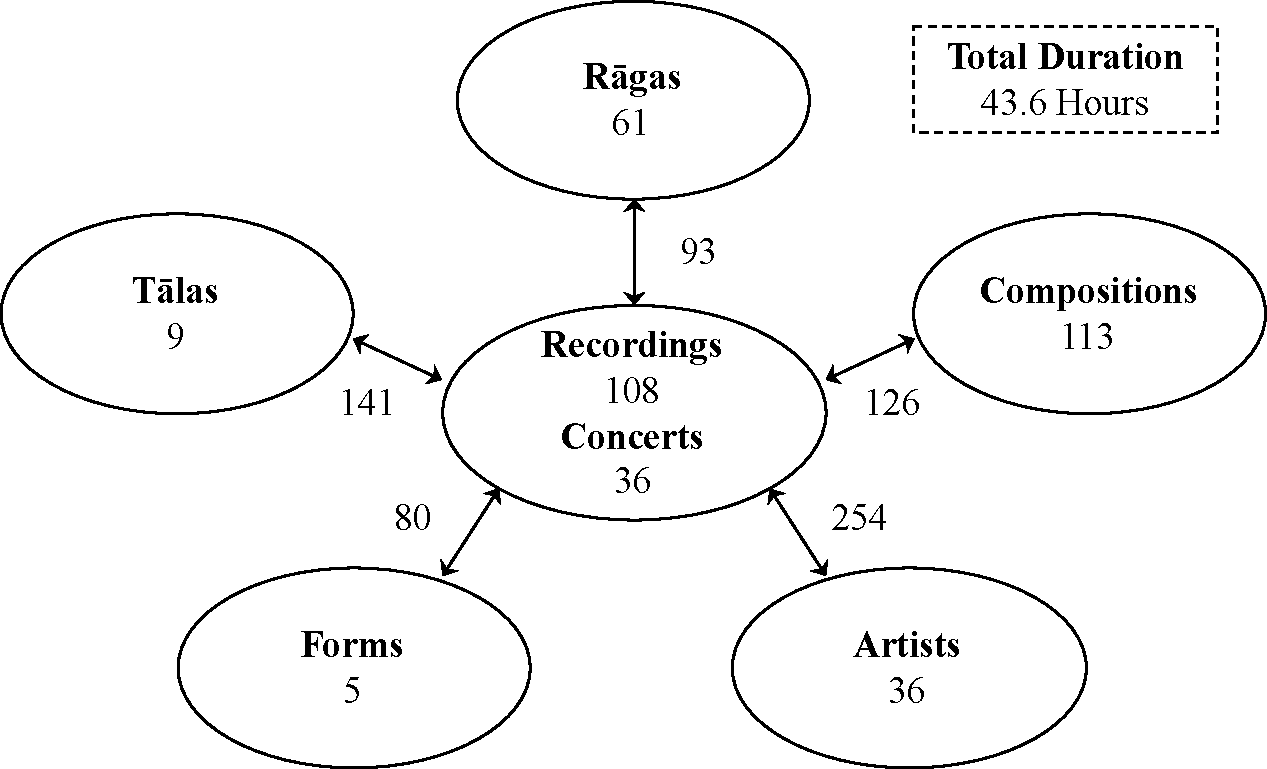
\includegraphics[width=\figSizeNinety]{ch04_datasets/figures/hindustani_corpus_cc.pdf}
	\end{center}
	\caption[Details of the Open-access Hindustani music corpus]{Details of the Open-access Hindustani music corpus in terms of the number of different musical entities and relationships between them}
	\label{fig:hindustani_cc_corpus_details}
\end{figure}


The audio recordings in both Hindustani and Carnatic music corpus are ripped from commercially released music CDs. The copyright on these recordings does not allow for a redistributed of the music content, and therefore, they cannot be made publicly available. Though these recordings are available in the market and are easily accessible, re-compiling the entire music corpus would practically require a lot of effort from a researcher who is trying to reproduce the research results. To promote the idea of open-access of research corpora and reproducibility of research results, in the CompMusic project there has been an effort to compile an open-access music collection. This open-access corpus comprises both Hindustani and Carnatic music. Like the other research corpora described in previous sections, this corpus contains audio recordings and associated editorial metadata. In addition, this corpus also contains several annotations of different music attributes such as melodic phrases, sama locations and sections. Due permissions are taken from the artists for redistribution of these audio recordings. As a result of which the corpus is made publicly available under creative commons license (CC BY-NC 4.0). The audio recordings in this corpus are hosted on Internet Archive\footnote{\url{https://archive.org/}} and made accessible through the Dunya Web \gls{api} (\secref{sec:applications_dunya}). 


\begin{figure}
	\begin{center}
		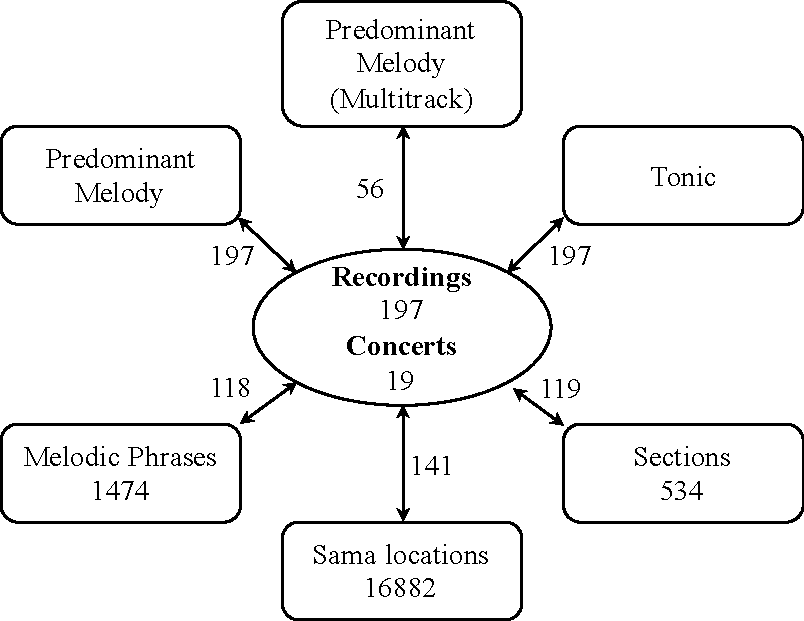
\includegraphics[width=\figSizeSeventyFive]{ch04_datasets/figures/carnatic_CC_details.pdf}
	\end{center}
	\caption[Details of the Carnatic open-access music corpus]{Details of the Carnatic open-access music corpus in terms of the number of available annotations of different musical attributes and audio features.}
	\label{fig:carnatic_open_access_corpus_details}
\end{figure}

The Carnatic music part of the open-access music corpus contains 19~releases comprising 197~recordings spanning over 41~hours of audio. A majority of these releases are recordings of Carnatic music concerts performed in the \gls{acc} in Chennai, India. These are multi-track recordings later mixed and mastered by a professional. Individual music pieces of a concert are split into separate recordings that then comprise a release. In addition to the content procured from the \gls{acc}, a number of releases in this corpus are commercially released CDs with artists' due permissions to make them publicly available. Along with the audio recordings and accompanying editorial metadata this corpus contains carefully done annotations corresponding to melodic, rhythmic and sectional aspects of the music. Manually done annotations include characteristic melodic phrases and sections within each audio recording. Semi-automatically done annotations include time-aligned sama locations and tempo in a recording. Finally, automatically done annotations, which can also be considered as mid-level audio features include predominant pitch contour and tonic frequency used in the recording by the lead artist. Since for several concerts their multi-track recordings are available, along with the predominant pitch estimated from the mix-down track we also compute pitch using the solo vocal track. These pitch contours from solo vocal tracks can serve as ground-truth data to evaluate pitch estimation algorithms for \gls{iam}. In \figref{fig:carnatic_open_access_corpus_details} we show the number of available annotations of different musical attributes and audio features for the Carnatic music part of the corpus.


\begin{figure}
	\begin{center}
		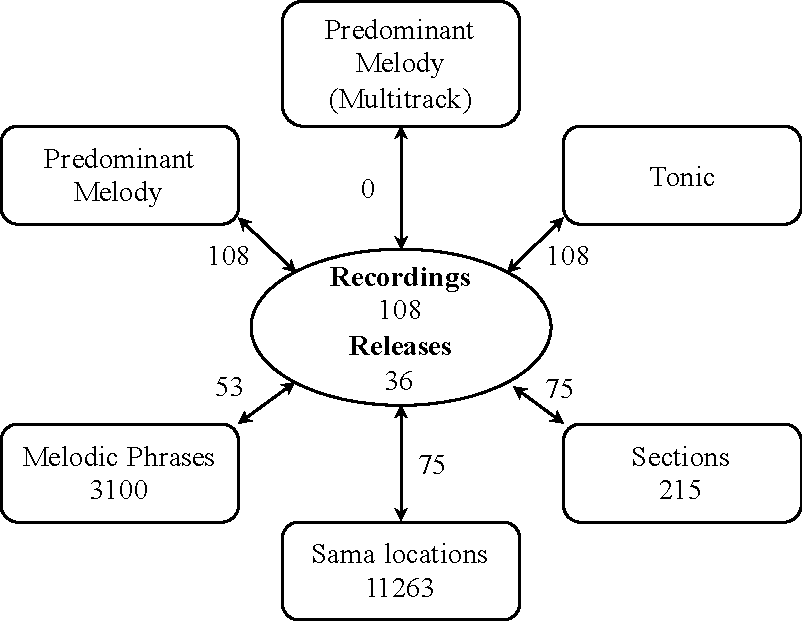
\includegraphics[width=\figSizeSeventyFive]{ch04_datasets/figures/hindustani_CC_details.pdf}
	\end{center}
	\caption[Details of the Hindustani open-access music corpus]{Details of the Hindustani open-access music corpus in terms of the number of available annotations of different musical attributes and audio features.}
	\label{fig:hindustani_open_access_corpus_details}
\end{figure}

The Hindustani music part of the open-access music corpus contains \TODO{XX} releases, which has \TODO{XX} number of recordings spanning \TODO{XX} hours of music. A significant portion of this collection comprises commercial releases by maestros such as Pt.~Ajoy Chakbraborty and Pt.~Kumar Gandharva. The other portion of the collection comprises individual recordings procured from different professional musicians and grouped together into meaningful releases for each artist. The grouping is based on common performance practices clubbing the performances in the \glspl{raga} that are performed together in a concert. This corpus also contains annotations for characteristic melodic phrases, sections, time-aligned sama locations and tempo. It also contain mid-level audio features including predominant pitch contour and tonic frequency used in the recording. Since multi-track recordings are available for this collection, pitch contours extracted from solo vocal track are not present. In \figref{fig:hindustani_open_access_corpus_details} we show the number of available annotations of different musical attributes and audio features for the Hindustani music part of the corpus. 



\subsection{Storage and Access of Corpus}
\label{sec:corpus_storage_and_access}

The previous sections described  various aspects of the Carnatic and the Hindustani research music corpus compiled in the CompMusic project. In this section we provide details on how the data in the corpus is storage and ways to access the data.

The audio corresponding to the corpora described above are largely stereo recordings sampled at 44.1\,kHz. For a few performances in the Carnatic open-access music corpus multi-track recordings are available. Most of the audio recordings in the corpora are ripped from the commercially released CDs. These recordings are compressed and stored as 160\,kbps MP3 files. The audio recordings for the open-access music corpus are hosted on Internet Archive. The rest of the audio recordings are hosted on the servers in Universitat Pompeu Fabra. In addition to the audio data, the corpora contain different melody and rhythm related audio features such as predominant pitch contours, tonic and tempo value of the music recordings. These features are also hosted on the university servers along with the audio recordings.

As mentioned, for every single audio recording in the corpora there is an accompanying editorial metadata. The metadata typically includes the following fields; lead artist, accompanying artists, instrument played by these artists, \gls{raga} and \gls{tala} of the music piece, music form and the name of the composition. For the case of Hindustani music it also includes \gls{laya} information. All this metadata is stored in the MusicBrainz, an open music encyclopedia. Every music concept in the MusicBrainz has a unique identifier, which facilitates the processing of this metadata. A number of complexities and problems arising from different spellings of an entity or different aliases of an entity are well handled by using this schema. There are several other advantages of using the MusicBrainz repository for storing editorial metadata, such as its ability to publish its database into Linked Data\footnote{\url{http://linkeddata.org/}}, mapping of entity concepts to Music Ontology\footnote{\url{http://musicontology.com/}}, its \acrshort{rest}-based webservice \acrshort{api} for direct access to its data. Above all, its a community driven open-content initiative and has its majority of the data in public domain.

All the data associated with a recording; the audio file, extracted set of features and the accompanying metadata can be accessed through the Dunya platform\footnote{\url{http://dunya.compmusic.upf.edu/}}. Dunya exposes this data in two ways; through a web-based graphical interface and through a \acrshort{rest}-based \acrshort{api}. A detailed description of the Dunya platform and the ways to access the data is provided in Section\TODO{secref}. Note that though the data is accessible for research purposes after user registration, not all the data in the corpora is in public domain. \TODO{what more?}



\section{Test Datasets}
\label{sec:corpus_test_datasets}

As explained earlier, a test dataset is a subset of a corpus used for studying a specific task. Typically a dataset is specific to an experiment and may contain additional information such as annotations. We here present the datasets that are used in different studies as a part of this dissertation. These datasets can be used for evaluating computational approaches for different melodic analyses in \gls{iam}. Some of these datasets are quite generic and contain good quality comprehensive editorial metadata along with the audio recordings. And hence, we envision their usage in other melodic analysis tasks beyond the ones addressed in this dissertation.

Since a majority of these datasets are a subset of the corpora described in previous sections, details regarding the quality of audio recordings and editorial metadata remain the same as that of the corpora. In case of exceptions, these details are provided in the section where the dataset is described. 


\subsection{Tonic Datasets}
\label{sec:corpus_tonic_datasets}


{\renewcommand{\arraystretch}{1.5}
\begin{sidewaystable} 
\begin{centering}
	\begin{tabular}{ c | c  c  c  c  c  c  c  c  c  c }
\tabletop
		Dataset 	&Avg. length (min)&\#Excerpts&	 	Hi.(\%) 	& 	Ca.(\%)	& 	Voc.
		(M/F)(\%) & Inst. (\%)	& 	\#Usong   	& 	\#Uartists	\\
\tablemid
		\acrshort{tds_cm1}		&3 &271	&	 41		& 	59	&	0			& 	100		& 	169		&	33	\\
		\acrshort{tds_cm2}		&3 &935	&	 45	 	& 	55	&	100 (68 / 32)		&	0		& 	547		&	81	\\
		\acrshort{tds_cm3}		&14.8&428	&	 45	 	& 	55	&	100 (72 / 28)		& 	0		&	428		&	71	\\
\hdashline
		\acrshort{tds_iitm1}		&144.6&38&	 0		& 	100	&	89 (79 / 21)		&	11		& 	N/A		&	22	\\
		\acrshort{tds_iitm2}		&12.3 &472	&	 0	 	& 	100	&	92 (77 / 23)		&	8		& 	472		&	22	\\
\hdashline
		\acrshort{tds_iisc}		&7.4&55	&	 0		& 	100	&	100 (80 / 20)		&	0		& 	55		&	5	\\
\tablebot
	\end{tabular}
	
	
	\caption[Summary of the tonic identification datasets]{Summary of the tonic identification datasets, including average excerpt length (Avg. length),
		number of excerpts (\#Excerpts), percentage of Hindustani music (Hi), Carnatic
		music (Ca), vocal excerpts (Voc.), instrumental excerpts (Inst.), number of
		unique songs (\#Usong) and number of unique artists (\#Uartists) in each dataset. For vocal
		excerpts we also provide the breakdown into male (M) and female (F)
		singers. Percentage (\%) values are rounded to the nearest integer.}
	\label{tab:tonic_datasets}
\par \end{centering}	
\end{sidewaystable}

We use six different datasets with varied characteristics for a comparative evaluation of approaches for tonic identification task in in \gls{iam}. The comparative evaluation is presented in \chapref{chap:data_preprocessing} and is based on our earlier work~\citep{Gulati2014Tonic}. Some of the tonic datasets overlap with the datasets used for evaluation in our earlier studies for the same task~\citep{salamon2012multipitch,gulati2012two}. A summary of the tonic datasets in terms of different attributes of the comprising excerpts such as their average length, their total number, proportion of Hindustani/Carnatic, instrumental/vocal and male/female excerpts, and unique number of songs and artists is provided in \tabref{tab:tonic_datasets}. In the subsequent paragraphs we describe each of these datasets in detail. Note that three out of the six datasets; \acrshort{tds_cm1}, \acrshort{tds_cm2} and \acrshort{tds_cm3} are compiled as a part of the work in this dissertation. 


\subsubsection{CompMusic Tonic Datasets}
\label{sec:corpus_compmusic_tonic_dataset}

The first three datasets shown in \tabref{tab:tonic_datasets}; \acrshort{tds_cm1}, \acrshort{tds_cm2} and \acrshort{tds_cm3} are tonic datasets compiled as a part of the CompMusic project. They are derived from the Carnatic and the Hindustani research corpus described in the previous sections. These datasets contain audio excerpts, associated metadata (lead artist, lead instrument, gender of the lead artist in case of a vocal performance) and tonic frequency annotation for every audio recording. The main differences across these three datasets are in terms of the duration of the excerpts and the type of music performance (vocal vs instrumental). These datasets comprise a diverse set of artists and music material such as gender of the singer, set of \glspl{raga} and music forms. Due to the diversity present in the datasets and the fact that these excerpts are taken from commercial releases, they can be regarded as a representative collection of \gls{iam} performances for tonic identification.  

\acrshort{tds_cm1} and \acrshort{tds_cm2} comprise three minute long audio excerpts extracted from full length recordings in the Hindustani and Carnatic music corpus. If a recording is longer than 12\,minutes, we extracted 3 excerpts from the beginning, middle and end of the recording. If the recording was shorter than 12\,minutes only one excerpt from the beginning was extracted. By taking excerpts from different sections of a song we ensure that the datasets are representative, since the musical characteristics can change significantly between different parts of a recording. \acrshort{tds_cm1} contains exclusively instrumental performances, and does not overlap with \acrshort{tds_cm2} and \acrshort{tds_cm3}. The latter two contain exclusively vocal performances, where \acrshort{tds_cm3} contains full performances and \acrshort{tds_cm2} contains excerpts taken from these performances. 

The tonic pitch for the vocal performances and tonic pitch-class for the instrumental performances was manually annotated for each excerpt. All the annotations were later verified by a professional Carnatic musician and the number of discrepancies was very small and later corrected. To assist the annotation process, we used the tonic candidate generation part of the approach proposed by \cite{salamon2012multipitch}. For every excerpt the top 10 tonic candidates were synthesized and played together with the original audio file to help identify and label the correct candidate. Note that the correct tonic pitch was always present amongst the top 10 candidates. A detailed description of this procedure is provided in~\cite{SGulati_MThesis2012}.


\TODO{A figure of tonic values in 428 + 169 performances}

\subsubsection{IITM Tonic Datasets}
\label{sec:corpus_iitm_tonic_datasets}

Datasets \acrshort{tds_iitm1} amd \acrshort{tds_iitm2} summarized in \tabref{tab:tonic_datasets} are compiled by~\cite{bellur2012knowledge}. These datasets were compiled by selecting 40 concerts from a private collection of hundreds of live concert recordings. These 40 concerts comprise 472 music pieces of Carnatic music. In order to study the robustness of tonic identification methods, the concerts that were selected range from artists from the 1960's to present day artists. The quality of the recordings vary from poor to good, usually depending on the period in which they were made. \acrshort{tds_iitm1} comprises 38 of these full-length concerts. \acrshort{tds_iitm2} comprises full length music pieces extracted from the 40 selected concert recordings. These performances are of varying duration, ranging from 46 seconds to 85 minutes. The tonic pitch for \acrshort{tds_iitm1} amd \acrshort{tds_iitm1} was manually annotated by a professional Carnatic musician.


\subsubsection{IISC Tonic Dataset}
\label{sec:corpus_iisc_tonic_dataset}

Dataset \acrshort{tds_iisc} is compiled by~\cite{ranjani2011carnatic}. It comprises audio recordings obtained from an online Carnatic music archive\footnote{\url{http://www.shivkumar.org/music/index.html}}. The archive is compiled by Carnatic musician and enthusiast Dr.~Shivkumar Kalyanaraman for the benefit of music amateurs and hobbyists as an online educational resource. The archive includes various forms of Carnatic music. \acrshort{tds_iisc} consists of 55 music pieces in the \gls{alapna} form, recorded by five singers across seven \glspl{raga}. The total duration of the dataset is 6.75\,hours. It includes recordings from the last 50 years, many of which were recorded live on analog audio tapes. The overall quality of the recordings is not very high. This makes it a challenging dataset for evaluating the accuracy of tonic identification approaches. The tonic pitch for recordings in this dataset was manually annotated by two professional musicians, S.~Raman and S.~Vijayalakshmi.


These six datasets represent the diversities present in real-world music collections of \gls{iam} in terms of the audio quality and music material, with which one can study the task of automatic tonic identification. To the best of our knowledge these are the largest and the most comprehensive datasets available for studying the task of tonic identification in \gls{iam}. \TODO{How can we obtain this dataset}



\subsection{Nyas Dataset}
\label{sec:corpus_nyas_dataset}

\Gls{nyas} dataset~(\acrshort{nds_cm}) is used for evaluating our proposed approach (described in \chapref{chap:data_preprocessing}) to identify \gls{nyas} \gls{svara} segments in melodies of \gls{iam}. \acrshort{nds_cm} comprises 20 audio music recordings of total duration of 1.5\,hours. All of these recordings are of vocal \gls{alap} performances of Hindustani music. \Gls{alap} is unmetered melodic improvisational, usually performed at the opening of a \gls{raga} rendition. We selected only \gls{alap} performances because the concept of \gls{nyas} is emphasized in these sections during a \gls{raga} rendition. Of the 20 audio recordings, 15 are polyphonic commercially available recordings taken from the Hindustani music research corpus (\secref{sec:corpus_hindustani_music_corpus}). The other 5 audio recordings in the data set are monophonic in-house studio recordings of the \glspl{alap} sung by a professional singer of Hindustani music. These in-house recordings are available under Creative Commons (CC) license in Freesound\footnote{http://www.freesound.org/people/sankalp/packs/12292/}. In total we have performances by 8 artists in 16 different \glspl{raga}. To avoid over-fitting of the data it is important to include different artists and \glspl{raga} as the \gls{nyas} characteristics highly depend on these aspects~\cite{Dey2008}.

\Gls{nyas} segments were annotated by a performing artist of Hindustani music (vocalist) who has received over 15 years of formal musical training. The musician marked all the \gls{nyas} segment boundaries and labeled them appropriately. This dataset contains 1257 \gls{nyas} \gls{svara} segments. The duration of these segments vary from 150\,ms to 16.7\,s with a mean of 2.46\,s and median of 1.47\,s.


%%Things to include in description
%1) What is the dataset for (which problem)
%2) Where is the problem addressed in this thesis. Which paper have we used this dataset in
%3) What are the other studies in which this is used
%4) Who compiled the dataset
%5) What does the dataset constitute (audio, metadata and what annotations)
%6) What is the musical characteristics of this data (vocal/instrumental, number of artists, number of songs, number of compositions, audio quality, music tradition, music forms)
%7) Possible table of different attributes of annotated data (length, stats etc)
%7) Annotation procedure followed

\subsection{Melodic Similarity Dataset}
\label{sec:corpus_melodic_similarity_dataset}

Melodic similarity dataset~(\acrshort{msds}) is built for evaluating approaches for computing similarity between short melodic fragments in \gls{iam}. Since the melodic characteristics across Carnatic and Hindustani music differ considerably, it is preferred to perform evaluations on each music tradition separately. Therefore, this dataset is divided into two parts; Carnatic music melodic similarity dataset (\acrshort{msds_iitm_cmd}) and Hindustani music melodic similarity dataset (\acrshort{msds_iitb_hmd}). Both these datasets contain audio recordings, bare minimum metadata (lead singer and \gls{raga} label for each recording) and time-aligned annotations of characteristic melodic phrases. \acrshort{msds_iitb_hmd} also contains predominant pitch estimated using a semi-automatic approach proposed by~\cite{rao2010vocal,rao2009applications}. \acrshort{msds_iitm_cmd} is compiled at DONLab in Indian Institute of Technology Madras, Chennai, India. This dataset was introduced by~\cite{Ishwar2013}, and since then it has undergone several changes. \acrshort{msds_iitb_hmd} is compiled at Digital Audio Processing Lab in Indian Institute of Technology Bombay, Mumbai, India. This dataset was introduced by~\cite{Ross2012b}, and has also undergone changes since then. Both these datasets have been used in several studies for a similar task~\cite{Ishwar2013, Ross2012b, Rao2014}\TODO{confirm if it was the same dataset used in other paper from IITB and IITM}.  We describe and share the version of these datasets used for the experiments done as a part of this dissertation (\TODO{chapter ref}), which are originally presented in~\cite{gulati_ICASSP2015,gulati_ISMIR_2015}.

\acrshort{msds_iitm_cmd} and \acrshort{msds_iitb_hmd} comprise polyphonic vocal music recordings of renowned artists in both Carnatic and Hindustani music. In \tabref{tab:melodic_similarity_dataset_details} we summarize the relevant details for both the datasets.  We see that these datasets are diverse in terms of the number of artists. 

{\renewcommand{\arraystretch}{1.5}
\begin{table} 
	\begin{centering}
		\begin{tabular}{ c | c c c c c}
\tabletop
			Dataset   	& 	Rec. 	&	PT		&	R\={a}gs	&	Artists		&	Duration\,(hr)\\	
\tablemid
			\acrshort{msds_iitm_cmd}   	& 	23 	&	5		&	5 	&	14		&	3.82\\	
			
			\acrshort{msds_iitb_hmd}   	& 	10 	&	5		&	2	&	8		&	1.92\\	
\tablebot
		\end{tabular}
		\caption[Details of the melodic similarity datasets]{Details of the melodic similarity datasets in terms of the total number of recordings~(Rec.), number of annotated pattern types~(PT), number of r\={a}gs, unique number of artists and total duration of the dataset.}
		\label{tab:melodic_similarity_dataset_details}
	\par \end{centering}
\end{table}

The melodic phrases in \acrshort{msds} are annotated by two professional musicians (one for each music tradition) who have received over 15 years of formal music training. All the annotated phrases are the characteristic melodic phrases of the \glspl{raga}. These characteristic melodic phrases are distinctly recognized by musicians, due to this fact the ambiguity involved in the judgment of melodic similarity is minimized to an extent. For both the datasets occurrences of five different melodic phrases are annotated. In \tabref{tab:categorywise_details_melodic_similarity_dataset} we summarize the relevant details for every category of the annotated melodic phrases for both the datasets. From the table we get an idea about the length of these phrases across their occurrences for each phrase type. In general, we see that the phrases in Hindustani music as compared to Carnatic music have a higher degree of variation in terms of their length. 

{\renewcommand{\arraystretch}{1.5}
\begin{table} 
	\begin{centering}
		\begin{tabular}{ c c|c c c c c c}
\tabletop
			Dataset	& PT 	&	\#Occ & $L_{\mathrm{mean}}$ & $L_{\mathrm{std}}$ &	$L_{\mathrm{median}}$ & $L_{\mathrm{min}}$ 	&	$L_{\mathrm{max}}$\\
\tablemid
		 \multirow{5}{*}{\acrshort{msds_iitm_cmd}} 
		
		 & $C_1$ & 31	&	1.41 & 0.24 &	1.44 &	0.99 	&	1.94	\\ 
		 & $C_2$ & 33	&	1.28 & 0.21 &	1.26 &	0.91 	&	1.91\\
		 & $C_3$ & 32	&	1.22 & 0.25 &	1.15 &	0.74 	&	1.71\\
		 & $C_4$ & 26	&	1.12 & 0.17 &	1.06 &	0.9 	&	1.6\\
		 & $C_5$ 	& 35&	0.75 & 0.09 &	0.74 &	0.63 	&	0.98\\
\tablemid
		 Overall	&  	& 157&	1.15 & 0.31 &	1.12 &	0.63 	&	1.94\\
\tabletop		 
		 \multirow{5}{*}{\acrshort{msds_iitb_hmd}} 
		 &  $H_1$ & 41	&	1.80 & 1.06 &	1.44 &	0.73 	&	5.26	\\ 
		 & $H_2$ & 139	&	1.33 & 0.74 &	1.22 &	0.38 	&	5.23 \\
		 & $H_3$ & 21	&	1.24 & 0.62 &	1.16 &	0.53 	&	2.82\\
		 & $H_4$ & 61	&	2.25 & 1.30 &	1.74 &	0.51 	&	5.93\\
		 & $H_5$ & 78	&	1.15 & 0.32 &	1.13 &	0.416 	&	2.64\\
\tablemid
		 Overall	&  	& 340 &	1.51 & 0.92 &	1.23 &	0.38 	&	5.93\\
 
					
\tablebot
		\end{tabular}
		\caption[Details of the annotated characteristic melodic patterns in \acrshort{msds} dataset.]{Details of the annotated characteristic melodic patterns in \acrshort{msds} dataset. PT:~phrase type, \#Occ:~number of annotated occurrences of  patterns of a PT, and $L_{\mathrm{mean}}$, $L_{\mathrm{std}}$, $L_{\mathrm{median}}$, $L_{\mathrm{min}}$ and $L_{\mathrm{max}}$ are the mean, standard deviation, median, minimum and maximum value of the lengths of the phrases of a PT.} 
		\label{tab:categorywise_details_melodic_similarity_dataset}
	\par \end{centering}
\end{table}

To correctly evaluate a method for an information retrieval task, it is important that the ground-truth annotations are complete, meaning that they cover all the occurrences of an object that the method aims to retrieve. Failing to do so might degrade the precision measurement of the method. In our case, wherein we evaluate the task of melodic similarity by casting it as a retrieval task, a similar situation exists. Along with the size of the dataset in terms of the number of melodic phrases, it is important that these annotations cover all occurrences of a melodic phrase. In \acrshort{msds} we discovered a number of discrepancies where several occurrences of the melodic phrases considered in this dataset were not annotated. When these cases were shown to musicians who annotated the dataset, they were surprised to know the errors in their annotations. Both the musicians commented that the possible reason why they missed marking such phrases was the melodic context in which these phrases are sung. When these phrases are played in isolation (without any melodic context) they appear to belong to the phrase categories considered in \acrshort{msds}. However, when played with the melodic context (i.e. including audio from a few seconds before the onset of the phrase) masks their identity and their identification becomes harder. Many such missed occurrences of the melodic phrases were added to \acrshort{msds} to build a revised version of the dataset, which we denote by \acrshort{msds_cm}. \acrshort{msds_cm} comprises exactly the same set of audio recordings as \acrshort{msds}. The only difference is in terms of the occurrences of the melodic phrases. In  \tabref{tab:categorywise_details_revised_melodic_similarity_dataset} we summarize the relevant details for every category of the annotated melodic phrases in both the datasets in \acrshort{msds_cm}. Comparing \tabref{tab:categorywise_details_melodic_similarity_dataset} and \tabref{tab:categorywise_details_revised_melodic_similarity_dataset} we notice that in the new dataset nearly 25\% of the melodic phrases are added. Note that the added annotations of the melodic phrases are verified by the same musicians who originally annotated the datasets.


{\renewcommand{\arraystretch}{1.5}
	\begin{table} 
		\begin{centering}
			\begin{tabular}{ c c|c c c c c c}
				\tabletop
				Dataset	& PT 	&	\#Occ & $L_{\mathrm{mean}}$ & $L_{\mathrm{std}}$ &	$L_{\mathrm{median}}$ & $L_{\mathrm{min}}$ 	&	$L_{\mathrm{max}}$\\
				\tablemid
				\multirow{5}{*}{\acrshort{msds_cm_cmd}} 
				& $C_1$ & 39 & 1.38 & 0.25 & 1.35 & 0.87 & 1.94\\
				& $C_2$ & 46 & 1.25 & 0.21 & 1.25 & 0.81 & 1.9\\
				& $C_3$ & 38 & 1.23 & 0.24 & 1.16 & 0.74 & 1.7\\
				& $C_4$ & 31 & 1.1  & 0.17 & 1.07 & 0.8  & 1.61\\
				& $C_5$ & 45 & 0.76 & 0.08 & 0.76 & 0.62 & 0.98\\
				\tablemid
				Overall	&  	& 199& 1.14 & 0.3  & 1.12 & 0.63 & 1.94\\
				
				\tabletop		 
				\multirow{5}{*}{\acrshort{msds_cm_hmd}} 
				&  $H_1$& 62	&	1.93 & 0.98	&	1.61 &	0.73	&	4.52\\
				& $H_2$ & 154 	& 	1.4  & 0.8 	& 	1.22 & 	0.38 	& 5.23 \\
				& $H_3$ & 47  	& 	1.3  & 0.8 	& 	1.08 & 	0.53 	& 4.49\\
				& $H_4$ & 76  	& 	2.38 & 1.34	& 	1.89 &	0.5  	& 5.93\\
				& $H_5$ & 87  	& 	1.17 & 0.37	& 	1.14 & 	0.42 	& 2.64\\
				
				\tablemid
				Overall	&  	& 426 & 1.6 & 0.99& 1.27 & 0.38 & 5.93\\
				
				\tablebot
			\end{tabular}
			\caption[Details of the annotated characteristic melodic patterns in \acrshort{msds_cm} dataset.]{Details of the annotated characteristic melodic patterns in \acrshort{msds_cm} dataset. PT:~phrase type, \#Occ:~number of annotated occurrences of  patterns of a PT, and $L_{\mathrm{mean}}$, $L_{\mathrm{std}}$, $L_{\mathrm{median}}$, $L_{\mathrm{min}}$ and $L_{\mathrm{max}}$ are the mean, standard deviation, median, minimum and maximum value of the lengths of the phrases of a PT.} 
			\label{tab:categorywise_details_revised_melodic_similarity_dataset}
			\par \end{centering}
	\end{table}
		
\subsection{\titlecap{\glsentrytext{raga}} Recognition Datasets}
\label{sec:corpus_raga_recognition_datasets}

\TODO{Do we need any motivation for building this dataset?}


\begin{figure}
	\begin{center}
		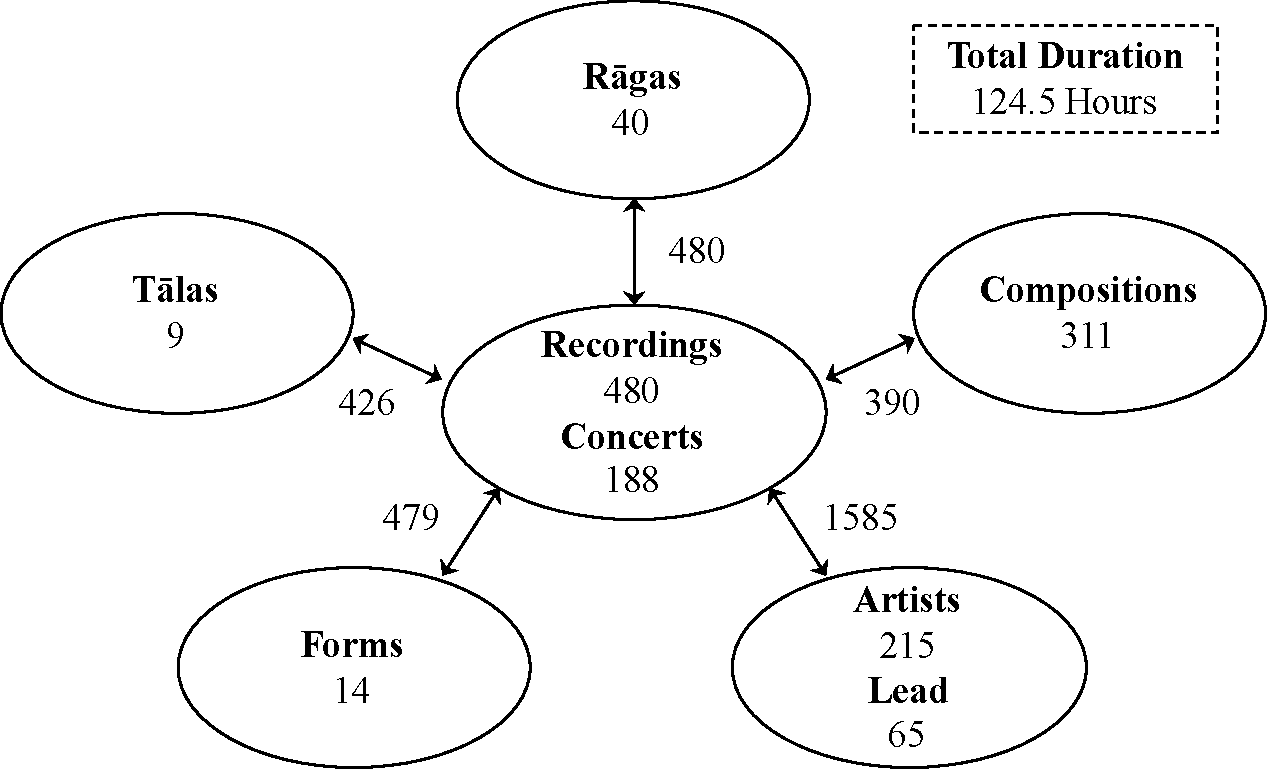
\includegraphics[width=\figSizeNinety]{ch04_datasets/figures/carnatic_corpus_ragaDB.pdf}
	\end{center}
	\caption[Details of the \gls{raga} recognition dataset comprising Carnatic music]{Details of the \gls{raga} recognition dataset comprising Carnatic music in terms of the number of different musical entities and relationships between them}
	\label{fig:carnatic_ragaDB_details}
\end{figure}

\begin{figure}
	\begin{center}
		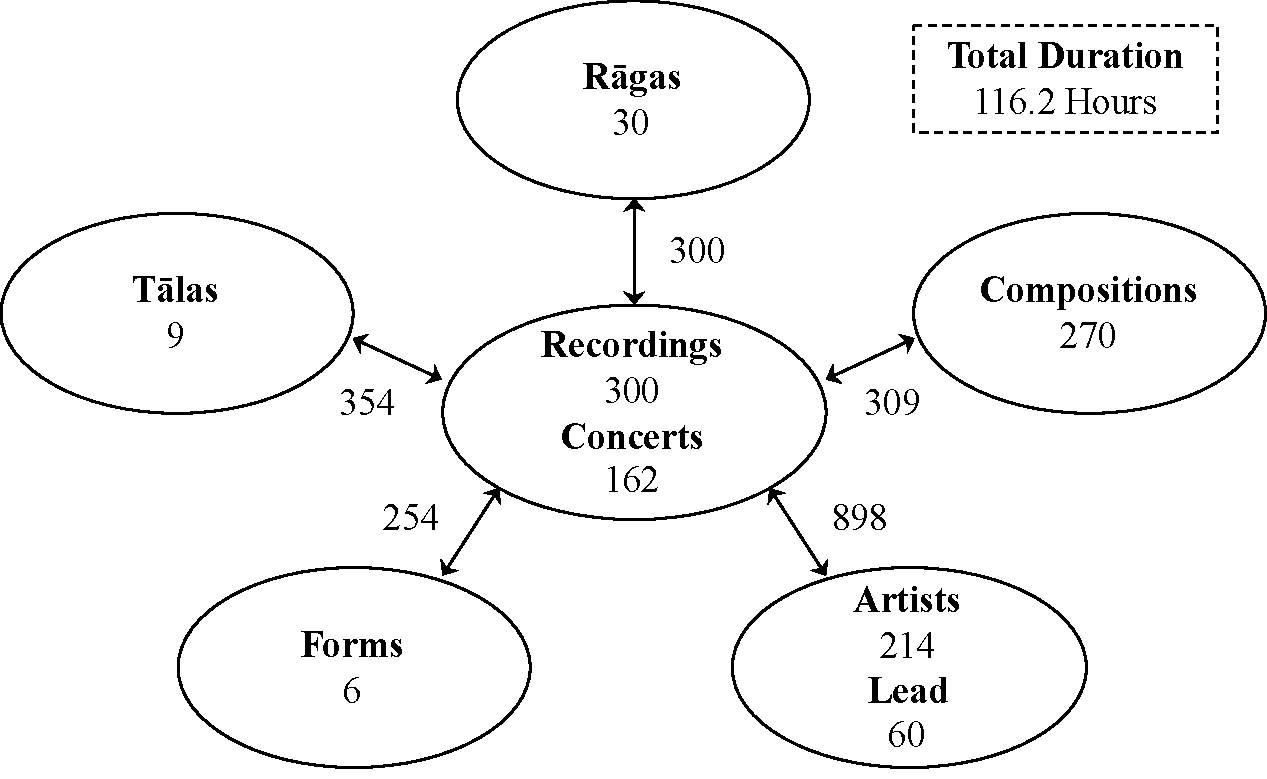
\includegraphics[width=\figSizeNinety]{ch04_datasets/figures/hindustani_corpus_ragaDB.pdf}
	\end{center}
	\caption[Details of the \gls{raga} recognition dataset comprising Hindustani music]{Details of the \gls{raga} recognition dataset comprising Hindustani music in terms of the number of different musical entities and relationships between them}
	\label{fig:hindustani_cc_corpus_details}
\end{figure}

As mentioned before, there are considerable differences in the melodic characteristics of Carnatic and Hindustani music. We therefore consider two separate datasets for evaluating approaches proposed for automatic \gls{raga} recognition~\chapref{chap:raga_recognition}. Carnatic music \gls{raga} recognition dataset (\acrshort{rrds_cmd_big}) is a subset of Carnatic music research corpus (\secref{sec:corpus_carnatic_music_corpus}) and is built as a part of the work done for this dissertation. \acrshort{rrds_cmd_big} was introduced in~\cite{gulatiphrase_2016}. \acrshort{rrds_cmd_big} comprises 124\,hours of audio recordings and editorial metadata that includes carefully curated and verified \gls{raga} labels. \acrshort{rrds_cmd_big} contains 480 recordings belonging to 40 \glspl{raga} with 12 recordings per \gls{raga}. This dataset primarily consists of vocal performances of 62 different artists. There are a total of 310 different compositions belonging to diverse forms in Carnatic music (for example k\={i}rtana, varnam, virtuttam). The chosen \glspl{raga} contain diverse set of \glspl{svara} (note), both in terms of the number of \glspl{svara} and their pitch-classes (\glspl{svarsthana}). Several selected \glspl{raga} share a common set of notes. This increases the complexity of the task, since the discrimination between these \glspl{raga} is mainly based on the temporal aspects of melody such as phrases and \gls{chalan} (\secref{sec:melody_in_iam}). To have diversity in the dataset we selected both phrase-based and scale-based \glspl{raga}.%In order to simulate the effect of small number of \glspl{raga} present in an evaluation dataset we also consider a subset of this dataset, denoted by \acrshort{rrds_cmd_small}. It contains 120 recordings belonging to 10 \glspl{raga}. \TODO{dataset detail, stats of the dataset + per raga stats and names of raga and svaras}

Hindustani music \gls{raga} recognition dataset (\acrshort{rrds_hmd_big}) is a subset of Hindustani music research corpus (\secref{sec:corpus_hindustani_music_corpus}) built as a part of the work done for this dissertation. \acrshort{rrds_hmd_big} was first introduced in~\cite{gulati_tdms_2016}. \acrshort{rrds_hmd_big} comprises nearly 130\, hours of audio recordings and editorial metadata. \acrshort{rrds_hmd_big} contains full-length recordings of 300~Hindustani music performances belonging to 30~\glspl{raga} with 10~music pieces per \gls{raga}. The selected music material is diverse in terms of the number of artists, the number of forms, and the number of compositions. \TODO{dataset detail, stats of the dataset + per raga stats and names of raga and svaras}

\acrshort{rrds_cmd_big} and \acrshort{rrds_hmd_big} can be regarded as representative subsets of real-world collections of \gls{iam}. To the best of our knowledge these are the largest and the most comprehensive (in terms of the available metadata) datasets ever used for studying the task of automatic \gls{raga} recognition. \TODO{How can we obtain these datasets}

\TODO{read description of these datsets in paper, see if you are missing something. PROVIDE A SUMMARY OF STATS, diff attributes. Musicbrainz editorial data etc!!}

\TODO{A table of all the ragas in bth the datasets and the svaras they comprise.}


\section{Summary}
\label{sec:corpora_summary}

\TODO{This summary is written in haste, try to rephrase it to make it intersting and use other words, also emphasize the contributions in this chapter!}

In this chapter, we described music corpora and test datasets that are compiled and curated as a part of our work within the CompMusic project. We enumerated the set of design criterion followed to gather and curate the corpora, and presented a brief evaluation of its goodness in terms of these criterion. We showed that the corpora contain representative audio collections of \gls{iam}. In addition to the corpora, we also described a number of test datasets used for evaluating different methods described in this thesis. To the best of our knowledge these are the largest corpora ever compiled for developing and testing data-driven computational approaches in the context of \gls{mir} in \gls{iam}. Both the corpora and the test datasets are made publicly available ensuring an easy accessibility of them.




